\documentclass[english]{lni}
\usepackage{graphicx}
\usepackage{booktabs}
\usepackage{tabularx}
\usepackage{array}
\usepackage{amsmath}
\usepackage{microtype}
\usepackage{placeins}
\addbibresource{Submission19_Koravi_SCIA_References.bib}
\begin{document}
\title{Sustainability Context Inheritance: From Trusted Evidence to Product Sustainability Profiles in Circular Economy Decision-Making}
\author[1]{Sandhya Koravi}{koravi.sandhya@gmail.com}{0009-0005-5087-793X}
\affil[1]{Lloyds Technology Centre\\Hyderabad, India}
\maketitle
\begin{abstract}
Circular economy decisions increasingly depend on sustainability evidence distributed across product passports, certifications, supplier disclosures, lifecycle assessments and regulatory systems. This paper introduces the Sustainability Context Inheritance Architecture (SCIA), a conceptual architecture for determining whether heterogeneous evidence is sufficient for a product-level sustainability claim in a specific Decision Context. SCIA links evidence to product structures, exposes Coverage Context and Sustainability Gaps, applies decision-specific attribution rules, and produces a Product Sustainability Profile (PSP). An illustrative electric-scooter case shows how weighted evidence coverage, explicit gaps and a mandatory assurance condition distinguish evidence availability from decision admissibility. The contribution is a decision-scoped, coverage- and gap-aware approach that reports claims as Supported, Partially Supported or Unsupported without treating evidence sufficiency as sustainability performance.
\end{abstract}
\begin{keywords}
Circular economy \and environmental informatics \and environmental decision support \and sustainability attribution \and decision context \and Digital Product Passport \and sustainability evidence \and Sustainability Lineage Graph \and Product Sustainability Profile
\end{keywords}

\section{Introduction}
European circular-economy policy and ISO guidance emphasize the transition toward sustainable and circular production \cite{EC20,IS24}. ESPR and DPP initiatives improve structured product-information availability and exchange \cite{EU24,CI24}; battery-passport guidance defines relevant passport content \cite{BP23}; and corporate sustainability reporting rules expand sustainability disclosure \cite{EU22}. However, information availability alone does not make a product-level claim decision-ready.

Evidence remains distributed across supplier declarations, certifications, product carbon footprints, lifecycle assessments, audits and proprietary systems. The European Commission reports that 53\% of assessed environmental claims were vague, misleading or unfounded and 40\% lacked supporting evidence \cite{EC23}. We refer to this decision problem as Environmental Information Asymmetry, extending information asymmetry to sustainability contexts \cite{Ak70}. SCIA asks a specific question: for a given sustainability claim and decision, is the available evidence sufficient, incomplete or missing?

SCIA is intended for decision roles such as OEMs, regulators, financial institutions, downstream actors and recyclers. In this paper, the Decision Context captures who is making or consuming the assessment (the actor) and the purpose for which the sustainability claim is being evaluated. Decision Context establishes the assessment scope; the Applicable Policy determines admissibility, materiality weights, mandatory conditions and thresholds.

The paper asks: RQ1: How can product-level sustainability claims be attributed from distributed evidence? RQ2: How can sufficiency, coverage limitations and evidence gaps be made explicit? RQ3: How can multi-organization and cross-jurisdiction evidence be consolidated into decision-ready PSPs?

The contribution comprises: (1) SCIA as an evidence-sufficiency architecture; (2) a Sustainability Lineage Graph linking product structures and evidence; (3) Coverage Context, Sustainability Gaps and Traceability Context as explicit sufficiency constructs; and (4) the PSP as a measurable, decision-scoped output reporting Supported, Partially Supported or Unsupported with supporting coverage, gaps and traceability. The contribution aligns primarily with SDG 9, SDG 12 and SDG 13.

\section{Related Work and Research Gap}
Existing sustainability mechanisms address complementary needs. DPPs provide structured mechanisms for associating product and lifecycle information with products and components \cite{EU24,CI24}; GS1 EPCIS provides cross-organizational visibility-event data that can support lineage and traceability \cite{GS1E}; GS1 Digital Link / Resolver connects identifiers to distributed resources \cite{GS1R}; and digital credential mechanisms such as verifiable credentials can carry machine-verifiable assertions together with issuer, validity and status information \cite{W3C25}. SCIA neither replaces nor depends on these mechanisms. Evidence may originate from them or from certifications, supplier disclosures and lifecycle assessments, with provenance and assurance metadata retained for later policy evaluation.

The research problem addressed by SCIA is specific: given heterogeneous and potentially incomplete evidence, is the evidence material to a particular product-level claim and decision sufficient to support that claim? SCIA represents the evidence through a Sustainability Lineage Graph, makes Coverage Context and Sustainability Gaps explicit, and applies Inheritance Assessment to produce a PSP. It is therefore a decision-oriented interpretation layer rather than another repository or traceability infrastructure; fitness-for-use research similarly emphasizes context rather than mere data existence \cite{WS96}. The remaining gap is how missing or incomplete decision-relevant evidence is measured and carried into product-level attribution, not merely how available evidence is represented or exchanged.

\begin{table}[ht]
\centering
\caption{Positioning of SCIA with complementary sustainability information mechanisms.}
\small
\begin{tabularx}{\textwidth}{>{\raggedright\arraybackslash}p{0.21\textwidth}>{\raggedright\arraybackslash}p{0.27\textwidth}X}
\toprule
\textbf{Mechanism} & \textbf{Primary role} & \textbf{Relationship to SCIA}\\
\midrule
Digital Product Passports & Structured product/lifecycle information & Potential sustainability-evidence source\\
GS1 EPCIS & Cross-organizational events/traceability & Potential event/lineage source\\
GS1 Digital Link / Resolver & Identifier resolution to distributed resources & Optional discovery mechanism\\
Trust/conformity mechanisms & Certification, validation, assurance & Can provide qualification/assurance information\\
SCIA & Decision-scoped evidence sufficiency/attribution & Produces PSP from relevant evidence, coverage, gaps and rules\\
\bottomrule
\end{tabularx}
\end{table}
\FloatBarrier

\section{Research Methodology}
This research follows Design Science Research (DSR) to design and evaluate a conceptual artifact addressing a socio-technical problem \cite{He04,Pe07}. The problem is Environmental Information Asymmetry; the artifact is SCIA and its Lineage Graph, Coverage Context, Sustainability Gaps, Inheritance Assessment and PSP; evaluation uses an illustrative electric-scooter scenario.

The evaluation is conceptual, examining internal consistency, gap visibility and decision discrimination through an author-defined policy instantiation. Decision Context scopes the claim and relevant evidence paths; the illustrative policy supplies materiality weights, admissibility requirements, mandatory conditions and thresholds. These parameters are neither universal nor empirically calibrated. Prototype performance, calibration, stakeholder validation and empirical decision-quality evaluation remain future work; SCIA remains metric-agnostic across product categories, domains and regulations.

\section{SCIA: Evidence Sufficiency Architecture}
SCIA asks whether available evidence is sufficient to support a sustainability claim for a particular decision. The Sustainability Lineage Graph maps evidence to product structures and lifecycle relationships; Coverage Context describes evidence completeness; Sustainability Gaps expose missing or unresolved evidence; and Traceability Context links evidence to its source and product path. These generic evidence-state constructs are interpreted during Context-Specific Inheritance Assessment using Decision Context and Applicable Policy, producing a PSP.

\begin{figure}[ht]
\centering
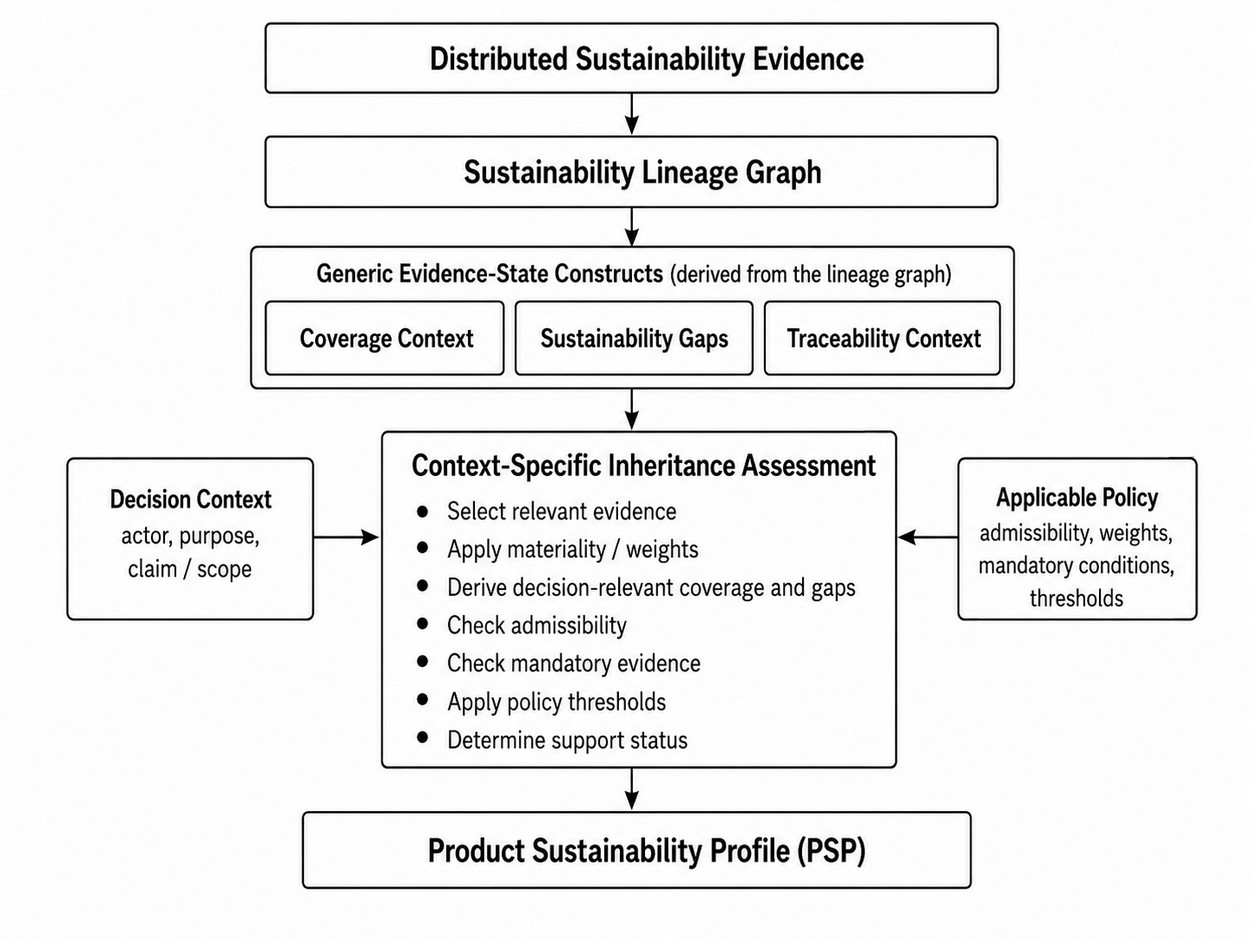
\includegraphics[width=.74\textwidth]{scia_extract/fig-000.png}
\caption{Sustainability Context Inheritance Architecture (SCIA).}
\end{figure}
\FloatBarrier

SCIA assesses evidence sufficiency, not sustainability performance, and does not prescribe how environmental metrics are calculated. Product carbon footprints or other metrics may be derived using applicable methods such as the GHG Protocol Product Standard \cite{WR11} or Product Environmental Footprint (PEF) \cite{EC21}. SCIA treats the resulting metric, methodological information and supporting evidence as inputs and assesses whether they are sufficient and admissible for the Decision Context and Applicable Policy. Its design principles are to trace evidence to source, make attribution explainable and expose rather than hide gaps.

\section{Mapping Evidence, Coverage and Gaps}
SCIA models the evidence landscape as a Sustainability Lineage Graph $G=(V,E)$, where $V$ includes Product, Component, Material, LifecycleStage, Evidence and Credential nodes, and $E$ includes relations such as contains, sourcedFrom, processedAt, evidencedBy and appliesTo. RDF or property-graph structures can represent the graph, with provenance, coverage and qualification information as attributes.

The graph supports three checks: what product/constituent structure is represented; what evidence and qualification information support each path; and where Sustainability Gaps remain. Evidence metadata may include provider or issuer, signer where applicable, product/component scope, provenance, validity or expiry status, and verification or assurance basis. Source-specific validation or verification results, where available, are retained as qualification metadata; SCIA does not replace those mechanisms. Such metadata does not prove the sustainability claim; it enables later admissibility assessment.

Coverage Context describes completeness of the available evidence landscape and may combine composition, evidence, lifecycle, assurance and provenance coverage; SCIA does not prescribe a universal generic formula. Sustainability Gaps identify missing, incomplete, inaccessible, unverifiable or unknown evidence and do not imply poor sustainability performance. Traceability Context links evidence and gaps to their source and product path.

\begin{figure}[ht]
\centering
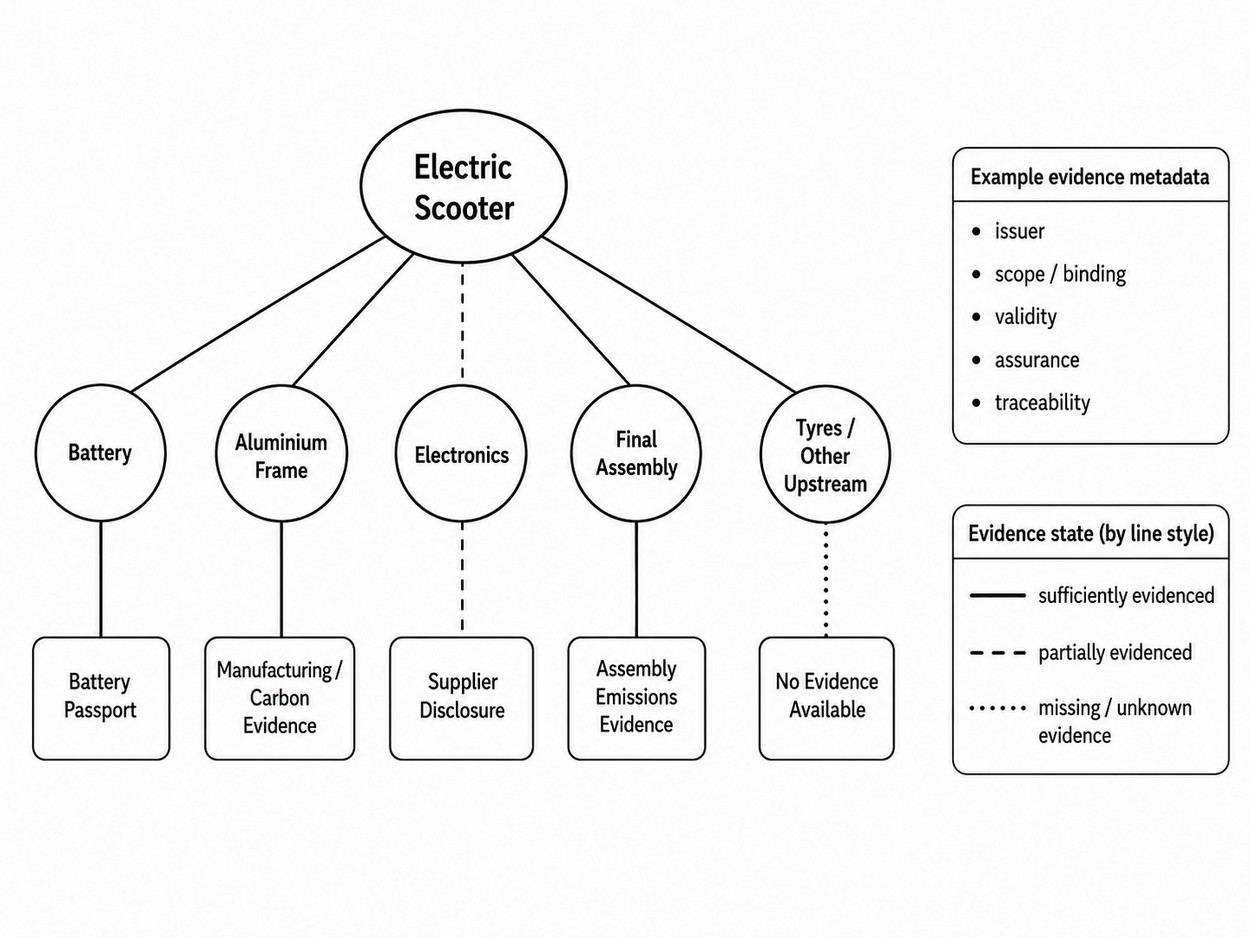
\includegraphics[width=.74\textwidth]{scia_extract/fig-001.png}
\caption{Sustainability Lineage Graph showing evidence coverage and Sustainability Gaps.}
\end{figure}

A practical SCIA implementation can remain technology-agnostic: evidence could be resolved from available sources and matched to product, component, process or lifecycle nodes using identifiers and semantic mappings, while provenance and qualification metadata are retained. GS1 Digital Link / Resolver can support resource discovery \cite{GS1R}, and EPCIS can provide visibility-event information for lineage \cite{GS1E}. The lineage itself may be represented using RDF or property graphs; SCIA does not require a specific implementation stack.

\section{Inheritance Assessment}
Inheritance Assessment interprets the generic evidence state for a Decision Context. For the illustrative low-carbon manufacturing assessment, let $c_i\in[0,1]$ be evidence coverage of relevant path $i$ and $w_i$ its policy-defined materiality weight, with $\sum_iw_i=1$. Decision-relevant coverage and gaps are:
\[
C_D=\sum_i w_i c_i \qquad g_i=w_i(1-c_i) \qquad G_D=\sum_i g_i.
\]
With normalized weights, $C_D+G_D=1$. These values quantify evidence sufficiency, not sustainability performance; weights represent decision relevance, not evidence reliability. Coverage measures the presence and completeness of decision-relevant evidence, but not whether that evidence satisfies the conditions under which a decision maker may rely on it. Evidence with identical coverage may differ in admissibility: policy may require independent assurance rather than self-attestation, an accepted accounting/assessment method, a recognized issuer or scheme, or a credential valid on the assessment date. SCIA therefore separates three questions: is relevant evidence available; is it admissible under the Applicable Policy; and is the admissible evidence sufficient for product-level inheritance? The gap terms $g_i$ and $G_D$ quantify evidence deficits; formal probabilistic uncertainty propagation remains future work. All values below are author-defined illustrations.

\begin{table}[ht]
\centering
\caption{Illustrative decision-relevant coverage and gap assessment.}
\small
\begin{tabularx}{\textwidth}{Xcccc}
\toprule
\textbf{Evidence path} & $\mathbf{w_i}$ & $\mathbf{c_i}$ & $\mathbf{g_i}$ & \textbf{Evidence state}\\
\midrule
Battery manufacturing & 30\% & 100\% & 0\% & Available\\
Aluminium/frame production & 20\% & 100\% & 0\% & Available\\
Electronics manufacturing & 25\% & 50\% & 12.5\% & Partial\\
Final assembly & 20\% & 100\% & 0\% & Available\\
Tyres/other upstream & 5\% & 0\% & 5\% & Unavailable\\
\midrule
Total & 100\% & $C_D=82.5\%$ & $G_D=17.5\%$ & --\\
\bottomrule
\end{tabularx}
\end{table}

The illustrative policy requires $C_D\geq90\%$ for Supported, $60\%\leq C_D<90\%$ for Partially Supported, and $C_D<60\%$ for Unsupported. Coverage alone therefore yields Partially Supported at $C_D=82.5\%$, with $G_D=17.5\%$ from electronics (12.5\%) and tyres/other upstream (5\%). This answers only how much decision-relevant evidence is available; it does not establish whether that evidence satisfies policy conditions for reliance on the claim. Section 7 applies those admissibility conditions and determines the final inheritance outcome.

\section{Illustrative Decision Assessment and Product Sustainability Profile}
The scenario asks whether an OEM has sufficient manufacturing evidence to substantiate, and therefore publish or rely on, a whole-product low-carbon manufacturing claim for an electric scooter. Section 6 established 82.5\% decision-relevant coverage. The second assessment step tests whether available evidence is admissible under the Applicable Policy and whether the admissible evidence permits whole-product inheritance. The illustrative OEM policy requires $C_D\geq90\%$ for Supported status and valid independent assurance for battery-manufacturing evidence from a provider accepted under the policy. This mandatory condition is author-defined for the illustration, not prescribed universally by SCIA.

Battery evidence is present, traceable and therefore 100\% covered in the lineage, but its qualification metadata shows that the required verification expired before the assessment date. Thus, evidence presence and coverage are distinct from decision-specific admissibility. The mandatory assurance failure overrides the coverage-based result and makes the final attribution Unsupported.
\[
\text{Mandatory admissibility condition failed}\Rightarrow\text{Unsupported}.
\]

\begin{figure}[ht]
\centering
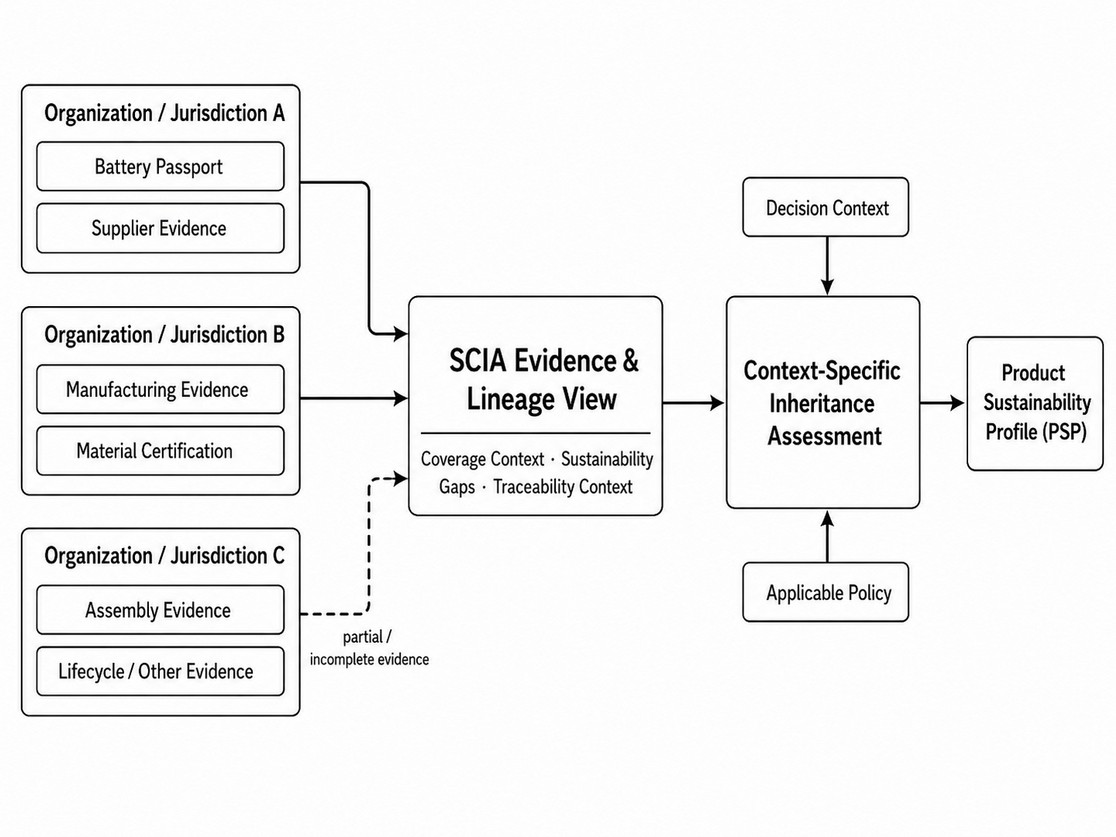
\includegraphics[width=.76\textwidth]{scia_extract/fig-002.png}
\caption{Federated sustainability evidence contributing to a decision-scoped PSP.}
\end{figure}

\begin{table}[ht]
\centering
\caption{Illustrative decision-ready Product Sustainability Profile.}
\small
\begin{tabularx}{\textwidth}{>{\raggedright\arraybackslash}p{.27\textwidth}X}
\toprule
\textbf{Decision information} & \textbf{PSP result}\\
\midrule
Claim being assessed & Manufacturing evidence is sufficient to substantiate a whole-product low-carbon manufacturing claim for the electric scooter\\
Decision & Whether the OEM should publish or rely on the claim\\
Applicable OEM policy & Supported: $C_D\geq90\%$; valid independent battery-manufacturing assurance is mandatory\\
Observed evidence state & $C_D=82.5\%$, $G_D=17.5\%$; battery evidence present and traceable, but required verification expired\\
Final PSP outcome & Unsupported - mandatory battery-assurance condition failed; coverage alone: Partially Supported\\
Key coverage gaps & Electronics manufacturing: 12.5\%; tyres/other upstream: 5\%\\
Required action & Obtain valid battery assurance and close remaining upstream gaps before reassessment\\
Traceability & Evidence, gaps and qualification status remain linked to product/component paths\\
\bottomrule
\end{tabularx}
\end{table}
\FloatBarrier

The PSP prioritizes the decision-blocking condition before diagnostic coverage detail. Because it is decision-scoped, the same evidence may yield a different outcome for another actor; for example, a recycler assessing end-of-life recoverability may apply different evidence paths, weights, mandatory conditions and thresholds. The scenario addresses RQ1 through lineage-based attribution, RQ2 through explicit coverage and gaps, and RQ3 through a decision-ready PSP. Numerical values and policy conditions are illustrative and demonstrate internal decision transparency, not empirical improvement in human decision quality.

\section{Limitations and Future Work}
SCIA is conceptual and does not claim prototype, empirical, stakeholder or expert validation. The scooter weights, thresholds and mandatory assurance rule are illustrative rather than universal or calibrated. SCIA also does not establish the substantive truth of evidence; it preserves provenance and assurance information while Applicable Policy determines admissibility. Practical deployments would need to integrate, as appropriate, with relevant mechanisms and account for DPP access and interoperability requirements \cite{EU24} and evidence validity or status changes such as credential revocation \cite{W3C25}. Attribution accountability remains a deployment concern.

As the next phase of this research, we plan to empirically evaluate SCIA using externally sourced product and sustainability evidence, including real-product prototyping and controlled evaluation of decision-specific coverage and admissibility conditions. Subsequent work will address calibration, stakeholder evaluation, formal uncertainty propagation, dynamic policy management and context-dependent evidence-path selection.

\section{Conclusion}
SCIA provides an evidence-sufficiency architecture for product-level sustainability attribution. The Sustainability Lineage Graph connects distributed evidence while preserving traceability and qualification information; Coverage Context and Sustainability Gaps expose evidence completeness and limitations; and Inheritance Assessment applies Decision Context and policy to determine decision-relevant coverage, admissibility and final status. The PSP reports the outcome, blocking conditions, gaps and traceability needed to understand the decision.

The OEM illustration shows that evidence may be present and traceable yet inadmissible when a mandatory assurance requirement fails. SCIA is therefore not another sustainability metric, evidence repository or trust mechanism, but a structured approach for determining whether evidence is sufficient and admissible for a product-level sustainability claim in a particular decision.

\printbibliography
\end{document}
